\chapter{水声传感网络MAC协议研究现状 }
\section{水声传感网络MAC协议分类}
\begin{figure}[ht]
	\centering
	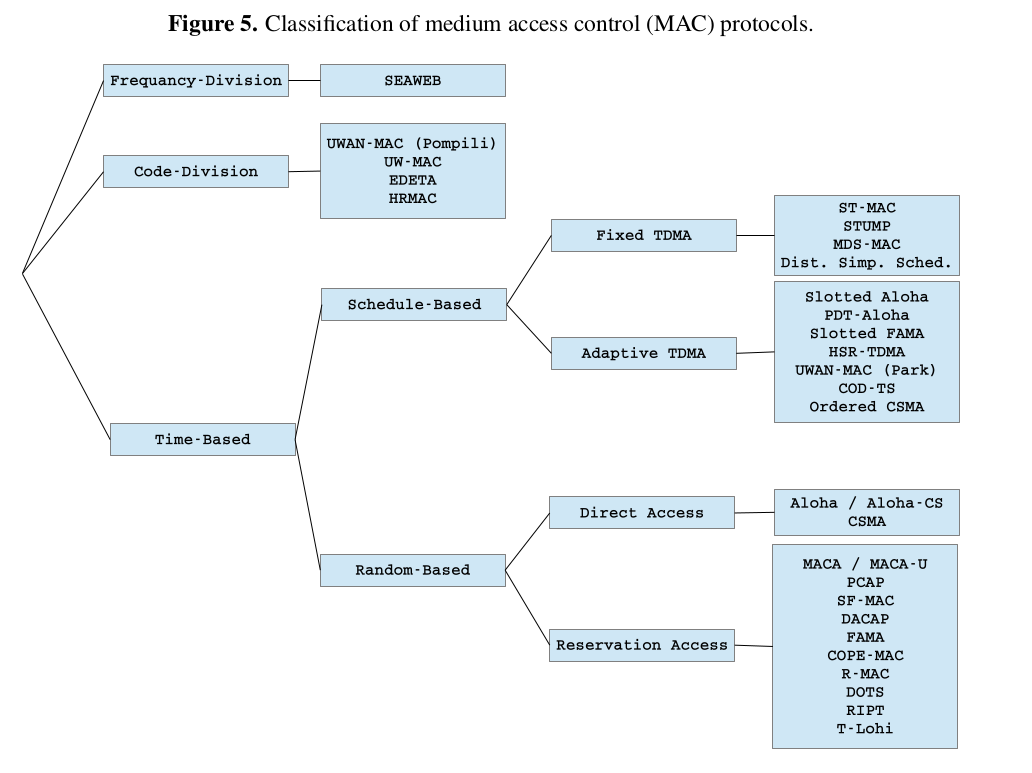
\includegraphics[scale=0.2]{figures/cha.png}
	\caption{
		水声传感网络
	}
	\label{fig:example}
\end{figure}
无线传感网络使用的MAC协议,通过信道占用方法可以分为竞争协议、非竞争协议和混合协议。竞争协议包括了ALOHA、载波侦听多址接入CSMA、基站捕获多址接入FAMA、冲突避免多址接入MACA等,非竞争协议包括了时分多址TDMA、码分多址CDMA、频分多址FDMA,混合协议包括了时空MAC(Spatial—Temporal MAC,ST-MAC)等。
\subsection{竞争协议}
基于Aloha的MAC协议有很多。纯A10ha协议非常简单:只要有节点想要发送数据,就立刻发送数据,无需考虑信道是否空闲。由于不侦听信道,会与正在发送中的数据包冲突,使得冲突节点发送的数据包被接收后都是无用的,而被丢弃。这种方式不仅降低了吞吐量,也浪费了能量。一个对纯Aloha改进MAC协议叫做Aloha—HD(Aloha谢tllHalfDu口lex,半双工A10ha协议)。Aloha-HD中,当节点意识到信道中的数据的目的节点是自己,该节点会一直保持接收数据模式,而不发送数据。如果信道中的数据不是发给自己,那么与纯A10ha一样,节点如果有数据发送可以立即发送。然而,Alolla一皿的前提条件是,能够接收到数据包的包头。Aloha另一个简单的变体是Aloha-CS(Aloha wi也CarrierSensillg,载波侦听Aloha协议)。Aloha.CS中要求只要信道中有数据,节点就不可以发送数据。然而,Aloha.cS不是侦听信道的状态,而是通过检测半双工的调制解调器是否在接收数据。Sl础ed.Aloha(时隙的Alolla)也被水下通
信考虑,即节点共享相同的同步时间,并且仅在时隙的开始时发送数据。然而在水下,
它的效率是低于在无线电中的效率。这是由于为了补偿不同的传输时延,需要长的保护
时间导致的。Nittllita Cllil.dchoo等人125J提出了Aloha的另外两个变种:Aloha.CA(Aloha
Notification,预知的Aloha协议)。这两个变体都利用节点从信道中收到的数据包,获
取数据包的发送端、接收端、以及发送端与接收端的时延,把侦听得到的信息添加到一
个数据库表中来避免冲突,以提高吞吐量。
载波监听多路访问(CSMA)代表了另一类的基于竞争的NoC协议。CsMA本身
要求数据包传输的时间应该远远大于传播延迟,然而在典型的水下网络是很难满足这个
条件的(由于水下大的延迟)。在水声传感器网络中直接使用CSMA会导致一个非常
长的漏洞时间。CS姒的另一形式在【26J中提出。在此,信道被侦听了一个很短的时间,
以避免一些必定产生冲突传输的模式。尽管可能是过于保守的行为【2‘71,其但性能良好。
冲突避免的CSMA(csMA.cA)也是一种选择。CSMA.CA以连接建立的更高的延迟
为代价减少冲突的机会。这是由于需要等待RTS/CTS交换的完成。水下带有数据包序
列的MACA在[28'29]中提出。DACAP(四)和APCAP【311就是CSMA—CA机制很好的例子。

然而,多跳拓扑结构可能导致控制包和数据包之间的碰撞。为解决这个问题,报文分片
【32】被提出。另一种方法是控制包单独使用一个信道【331。【34】进一步扩展,使用多信道进
行数据通信。时间槽的FAl、压A(Slo地d—FAMA)【35]是基于为陆地传感器网络设计的
FAMA【36l协议的改进。FAMA协议将时间分槽,载波侦听和握手技术结合在一起。
Slotted.FA讹~的主要原理与CSMA很相似,但Slotted.FAMA把时间划分成时间片,并
且要求节点只能在时间片的开始时发送数据包或者控制包如果一个节点想要发送数据
包,该节点必须等到下一时间片的开始,然后才能开始它的CSMA过程。Slo讹d.FAMA
基本上是融合了CsMA和Slo讹d-A10ha。为提高网络的性能,另一个想法就是重用。
R口T【3刀和DOST【381通过限制发送端而重用信道。MFAMA【39】允许发送者和多个接收者之
间发起多个会话。发送者利用偷听到的信息计算邻居节点之间的会话安排,以选择合适
的发送数据的时间。T.Lolli【15】是一个基于预留机制的竞争MAC协议。节点竞争信道的
使用权,然后发送数据。每个时间帧包含若干个争用回合(CR,Contention RouIld)和
一个无竞争的数据发送时间段。在竞争阶段,要求节点在CR时发送一个tone信息,然
后侦听信道来判断是否竞争成功。如果只有该节点竞争信道,那么该节点在接下来的数
据时间段(DP,Data Period)发送数据.如果多个节点在同一个CR竞争信道,那么每个
节点都会检测到竞争。然后这些竞争的节点会回退。在接下来的某个cR重新竞争信道。

\subsection{非竞争协议}
基于固定分配的MAC协议有频分多路复用、时分多路复用、码分多址复用。
频分多路复用(FDMA,Frequency
DiVision
Muhiple Access)把信道划分为若干个
子信道,然后把子信道分配给指定的节点使用。只有节点放弃使用子信道时,其他节点
才可以使用。虽然FDNo在陆地无线网络的性能很好,但由于水声信道的可用带宽窄,
如果把信道划分成小的子信道,传输信道的相干带宽可能大于子信道的带宽。相应的,
会造成使用不同子信道的节点的衰减[401。特别是,如果在数据量大的水声传感器网络中,
由于子信道是固定分配给节点的,不具有适应动态变化的网络环境的能力,因此,FDMA
的性能会低下14H21。
时分多路复用(II)MA,Time
Division
Multiple Access)是把时间划分为时间片而
分给节点的接入方法。一个时间片只分配给一个用户使用,每个节点只在给定的时间片
传送数据。在陆地网络中,有很多使用II)MA技术,如GSM(Global
[43】,Is 136
System
ofMobil姆)
m】。然而,TI)m为了避免节点之间分配的时间片有冲突,必须在时间片之
间加入一个短的时间片,即保护时间(guard time),这个开销比FDMA还要大【451。另
一个缺点是水下环境的长传输时延使得TDMA时间同步很难实现。因此会发生数据冲
突,降低系统性能。
与FDMA、TDMA不同,码分多址复用(CDMA,Code
DiVision
MmtiDle Access)
并不划分时间和带宽,而是允许所有节点同时在同一个信道上发送数据。通过给每个节
点分配不同的扩频码来区分节点。这些扩频码是相互正交的。CDMA有两种类型:直接
序列扩频(DSSS,Direct
sp佗ad
Sequence Spread
Specmlm),跳频扩频(FHSS,Frequency-hopping
specm皿,FHSS)。

\subsection{混合协议}
针对水声传感网络调制解调器存在多种模式和多种传输速率等特点,文献1961提出了适
用于多模式多速率水声传感网络调制解调器的自适应MAC协议。仿真和海洋试验结果表
明,该协议能很好地适应水声传感网络环境,达到较好的网络性能。针对压缩感知应用的
水声传感网络,文献【97】根据节点数和有效数据还合理分配时隙,提高网络数据传输效率
和能量效率。文献【98】针对水声传感网络信遒衰落与节点距离的关系,提出了发送功率与
速率自适应的MAC协议,通过合理控制不同节点距离之间的信号功率和速率,达到较好
的网络吞吐量和能耗性能。
长延时网络MAC(MAC
Protocol for Long-latency Access
Networks,PLAt,0协议(99J是综
合CDMA和RTS/CTS三次握手交互方式的混合MAC协议。在网络初始化阶段,各节点
预先被分配了正交的扩频码作为地址码,在后续的通信过程中,各节点使用该扩频码来发
送数据。针对水声传感网络长传播时延的特点,一个节点可能在一定时间内收到多个RTS,
不同于陆地无线网络MAC协议认为有冲突的做法,PLAN在这些RTS中随机选取一个RTS
作为发送端并返回CTS,当对应的发送端接收到Crs后,知道已经被选中则开始发送数据。
该协议有利于提高RTS和CTS数据交互的成功,降低了节点接收到多个RTS时认为冲突
导致的信道资源的浪费,提高了信道利用率。文献[100]提出了基于CDMA和ALOHA的
分布式MAC协议,考虑到网络各节点固定分配扩频码时需要较长的码长,该协议对各节
点的扩频码进行动态分配,只对当前要进行通信的节点进行分配扩频码,使得扩频码长得
到了很大的降低,提高了网络信道利用率。

\section{移动水声传感网络MAC协议研究现状}
根据移动水声网络的分布式特性和可扩展性,Francisco Salvá-Garau和Milica Stojanovic提出了多集群(Multi-CLuster)\cite{Multi-Cluster Protocol for Ad Hoc Mobile Underwater Acoustic Networks Oceans2003}MAC协议。将邻近节点分在一个集群中,在单个集群内使用统一的TDMA协议通信。不同集群间通过分配不同的扩频码来减少串扰、提高扩展性。协议分为两个阶段,首先在初始化阶段分配不同集群,然后是持续时间较长的稳定传输阶段。

考虑到移动水声网络的低速率特性,Youngtae Noh和Uichin Lee等在2014年提出了DOTS(A Propagation Delay-Aware Opportunistic MAC Protocol for Mobile Underwater Networks)协议。通过被动获得的本能信息,如邻居节点传播时延表以及预期调度时序等,实现同一信道上多数据包并行发送。\cite{DOTS: A Propagation Delay-Aware Opportunistic MAC Protocol for Mobile Underwater Networks}

对于有移动节点接入的小规模单跳传感网络,毛佳、徐元欣等提出了LTM-MAC(Location-based TDMA MAC protocol for mobile underwater networks)\cite{LTM-MAC: A location-based TDMA MAC protocol for mobile underwater networks}协议,给移动节点的接入分配了较高的优先级。对于移动节点接入的小规模多跳传感网络,提出了TMM-MAC协议(TDMA-based MAC for Multiple-hops in mobile underwater networks)。利用多跳特性,允许与移动节点互不干扰的固定节点并行发送数据,同时根据数据包长短设计不同的发送机制。

基于移动节点进行数据收集的情景,邓敏、陈惠芳等人提出了混合MAC协议\cite{A Hybrid MAC Protocol in Data-collection-oriented
	Underwater Acoustic Sensor Networks},在低负载的子网中采用基于竞争的CT-MAC(ConTention-based MAC),在高负载的子网中采用基于轮询调度的RSV-MAC(ReSerVation-based MAC)。



\endinput